\cleardoublepage
\chapter{MATs}
\label{ch:8}
 
%------------------------------------------------

\section{Introduction}

\begin{fullwidth}
Material Operators, or MATs, are used for materials and shaders for 3D geometry.

A deep knowledge of computer graphics and rendering helps a great deal when working with materials and shaders. Without this knowledge, most users will be restricted to the basic settings of the Phong MAT and Point Sprite MAT.

Texturing and UV mapping geometry are involved processes, and the best results are often achieved inside dedicated modelling packages. The textured models can then be imported, and worked with, in TouchDesigner. 

Many tools exist for modifying textures, such as the Texture SOP, but complex processes might be easier to achieve in a software package created for that specific purpose.

\end{fullwidth}

%------------------------------------------------

\section{Phong, GLSL, and Point Sprite Materials}

\begin{fullwidth}

The three most used MATs are:

\begin{itemize}
\item the Phong MAT
\item the GLSL MAT
\item the Point Sprite MAT
\end{itemize}

The general uses of these three MATs will quickly be covered in this section. These are three very different Operators, and cover many shading and material needs.

The Phong MAT is the most common material Operator. It is responsible for applying texture to 3D geometry. There are a variety of maps that can be applied, such as Color, Bump, Specular, Diffuse, and more. The Phong MAT can mix and match Ambient, Diffuse, Specular, Emit, and Constant lighting. Open example 'Phong.toe'. In this project there are two very simple examples of the Phong MAT. The first uses the texture's alpha to create a transparent box. The second sets the Emit Light of 1,1,1 to fully illuminate the object regardless of the lighting condition. There will be many examples of the Phong MAT when it is put to use the examples section.

The GLSL MAT is used to create custom materials using the OpenGL Shading Language (GLSL for short). GLSL is a fantastic programming language that can create extremely complex textures that run extremely quickly. It achieves this by giving the programmer quite a bit of control over the graphics pipeline, without exposing them to assembly languages. There can be a slight learning curve when first starting, but there are tons of examples of GLSL shaders on the Internet, as well as quite a number of great examples in the 'Shared Component' area of the TouchDesigner Forum.

The Point Sprite MAT is used to assign sprites to the points of a particle system. The name is self explanatory, in that a 2D image (a sprite) is placed at every single point in 3D space. The sprites are always facing the camera, and are scaled according to their Z depth. The example 'Point\_Sprite.toe' demonstrates this. To create a similar TouchDesigner network without point sprites, not only would there be a pretty disorganized Network, of who knows how many Transform TOPs and Composite TOPs, but they would all be using much more resources. By using a particle system and point sprites, the Network is easy to read, and doesn't require a lot of system resources.
\end{fullwidth}

%------------------------------------------------

\section{UV Maps}

\begin{fullwidth}

UV mapping is an essential to working with complex 3D geometry. As with certain other aspects of 3D modelling, it is easier to create and work with UV maps in a dedicated modelling program.

UV mapping is what allows designers and artists to create interesting motion and still graphic textures for 3D geometry. It bridges the 2D world that motion and still graphics are created in with the 3D world of the geometry. 

UV mapping is a three-step process. The first step is the unwrapping of the 3D object into a 2D plane. This unwrapped texture is called a UV map. It is referred to as a map, because much like any other type of map, it takes a 3D object and accurately, and proportionally, creates a 2D reference. This is the same as street maps or world maps, that take the 3D universe and represent them on a 2D plane.

Texturing is the the second step. The 2D UV map is used by artists and designers in their compositing softwares to create textures, whether still or moving. The benefit of the UV map is that the textures can be applied to the geometry with a high degree of precision.

The third step is the application of the texture onto the 3D geometry. This varies depending on the software used.

The combination of these three steps are referred to as UV mapping.

The third step is a relatively common operation in TouchDesigner. As long as the 3D geometry is exported correctly from its modelling software, it will include co-ordinates indicating to other applications where the UV maps should be applied. In these situations the texture is loaded in a Movie In TOP and applied using a Phong MAT to the geometry. If any changes need to be made to how the UV map is applied, the Texture SOP can be used. 

Below is an example of a simple 3D box, and it's UV map:

\begin{center}
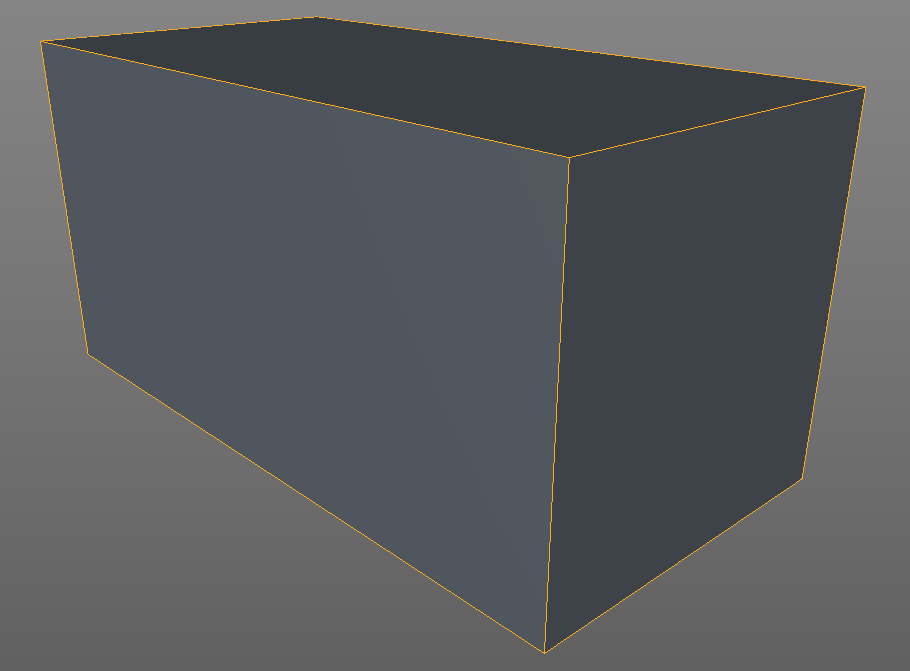
\includegraphics[width=15cm]{./img/8.3/3D-geo.png}

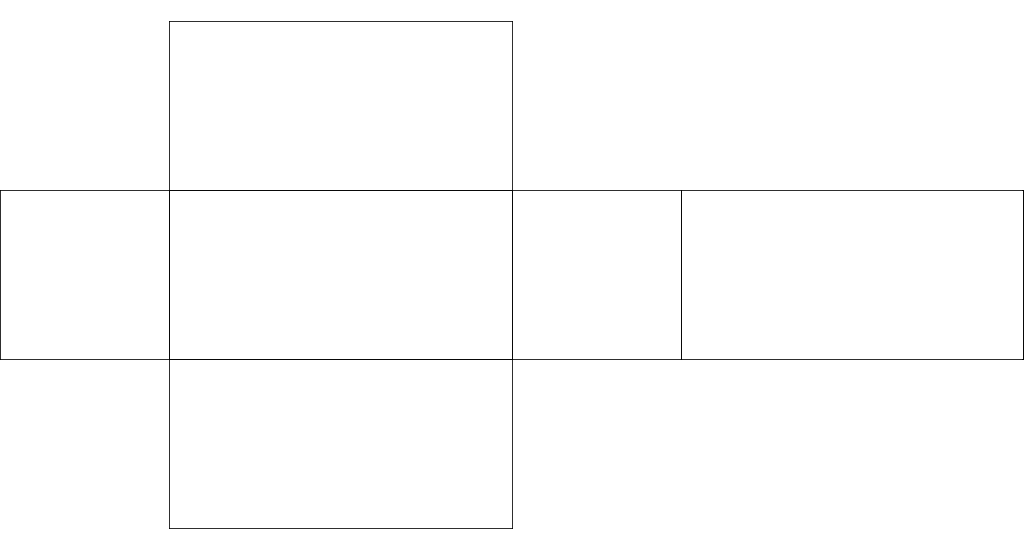
\includegraphics[width=15cm]{./img/8.3/Geo-map.png}
\end{center}

\end{fullwidth}
